Dans Scrum, trois rôles principaux sont définis :

\begin{itemize}
    \item \textbf{Product Owner} : Représentant des parties prenantes, il définit et priorise les fonctionnalités à développer en fonction des besoins des utilisateurs et des objectifs du projet.
    \item \textbf{Scrum Master} : Responsable de la bonne application du framework Scrum. Il facilite la communication, aide à surmonter les obstacles et veille à l'amélioration continue des processus.
    \item \textbf{Équipe de développement} : Composée de développeurs, designers et autres spécialistes, elle est responsable de la mise en œuvre des fonctionnalités et de la livraison des incréments du produit.
\end{itemize}

En adoptant Scrum, le projet bénéficie d'une approche structurée et efficace, garantissant un suivi rigoureux et une réponse rapide aux exigences changeantes du domaine médical.

\begin{figure}[H] % Use [H] to force the figure to appear exactly here
    \centering
    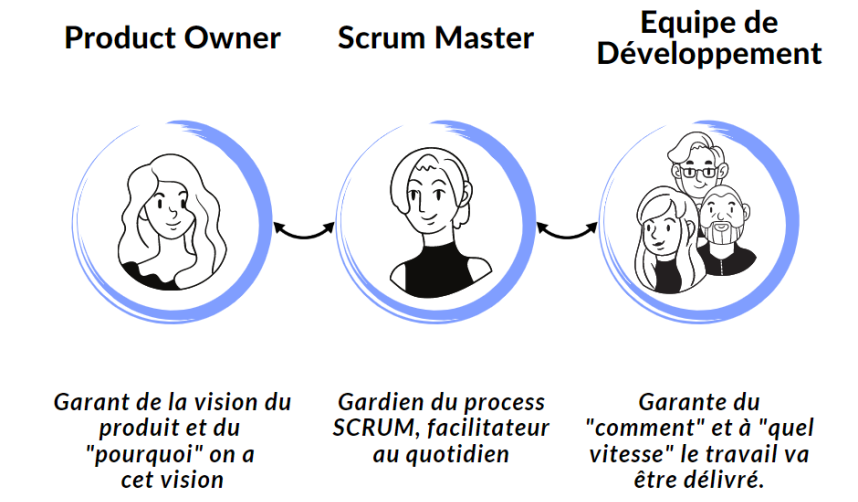
\includegraphics[width=1\linewidth]{chapter1/images/scrum-roles.png} % Adjust width as needed
    \caption{Rôles Scrum}
    \label{fig:scrum_roles}
\end{figure}